\documentclass[]{article}
\usepackage{lmodern}
\usepackage{amssymb,amsmath}
\usepackage{ifxetex,ifluatex}
\usepackage{fixltx2e} % provides \textsubscript
\ifnum 0\ifxetex 1\fi\ifluatex 1\fi=0 % if pdftex
  \usepackage[T1]{fontenc}
  \usepackage[utf8]{inputenc}
\else % if luatex or xelatex
  \ifxetex
    \usepackage{mathspec}
  \else
    \usepackage{fontspec}
  \fi
  \defaultfontfeatures{Ligatures=TeX,Scale=MatchLowercase}
\fi
% use upquote if available, for straight quotes in verbatim environments
\IfFileExists{upquote.sty}{\usepackage{upquote}}{}
% use microtype if available
\IfFileExists{microtype.sty}{%
\usepackage{microtype}
\UseMicrotypeSet[protrusion]{basicmath} % disable protrusion for tt fonts
}{}
\usepackage[margin=1in]{geometry}
\usepackage{hyperref}
\hypersetup{unicode=true,
            pdftitle={Recitation1},
            pdfborder={0 0 0},
            breaklinks=true}
\urlstyle{same}  % don't use monospace font for urls
\usepackage{color}
\usepackage{fancyvrb}
\newcommand{\VerbBar}{|}
\newcommand{\VERB}{\Verb[commandchars=\\\{\}]}
\DefineVerbatimEnvironment{Highlighting}{Verbatim}{commandchars=\\\{\}}
% Add ',fontsize=\small' for more characters per line
\usepackage{framed}
\definecolor{shadecolor}{RGB}{248,248,248}
\newenvironment{Shaded}{\begin{snugshade}}{\end{snugshade}}
\newcommand{\AlertTok}[1]{\textcolor[rgb]{0.94,0.16,0.16}{#1}}
\newcommand{\AnnotationTok}[1]{\textcolor[rgb]{0.56,0.35,0.01}{\textbf{\textit{#1}}}}
\newcommand{\AttributeTok}[1]{\textcolor[rgb]{0.77,0.63,0.00}{#1}}
\newcommand{\BaseNTok}[1]{\textcolor[rgb]{0.00,0.00,0.81}{#1}}
\newcommand{\BuiltInTok}[1]{#1}
\newcommand{\CharTok}[1]{\textcolor[rgb]{0.31,0.60,0.02}{#1}}
\newcommand{\CommentTok}[1]{\textcolor[rgb]{0.56,0.35,0.01}{\textit{#1}}}
\newcommand{\CommentVarTok}[1]{\textcolor[rgb]{0.56,0.35,0.01}{\textbf{\textit{#1}}}}
\newcommand{\ConstantTok}[1]{\textcolor[rgb]{0.00,0.00,0.00}{#1}}
\newcommand{\ControlFlowTok}[1]{\textcolor[rgb]{0.13,0.29,0.53}{\textbf{#1}}}
\newcommand{\DataTypeTok}[1]{\textcolor[rgb]{0.13,0.29,0.53}{#1}}
\newcommand{\DecValTok}[1]{\textcolor[rgb]{0.00,0.00,0.81}{#1}}
\newcommand{\DocumentationTok}[1]{\textcolor[rgb]{0.56,0.35,0.01}{\textbf{\textit{#1}}}}
\newcommand{\ErrorTok}[1]{\textcolor[rgb]{0.64,0.00,0.00}{\textbf{#1}}}
\newcommand{\ExtensionTok}[1]{#1}
\newcommand{\FloatTok}[1]{\textcolor[rgb]{0.00,0.00,0.81}{#1}}
\newcommand{\FunctionTok}[1]{\textcolor[rgb]{0.00,0.00,0.00}{#1}}
\newcommand{\ImportTok}[1]{#1}
\newcommand{\InformationTok}[1]{\textcolor[rgb]{0.56,0.35,0.01}{\textbf{\textit{#1}}}}
\newcommand{\KeywordTok}[1]{\textcolor[rgb]{0.13,0.29,0.53}{\textbf{#1}}}
\newcommand{\NormalTok}[1]{#1}
\newcommand{\OperatorTok}[1]{\textcolor[rgb]{0.81,0.36,0.00}{\textbf{#1}}}
\newcommand{\OtherTok}[1]{\textcolor[rgb]{0.56,0.35,0.01}{#1}}
\newcommand{\PreprocessorTok}[1]{\textcolor[rgb]{0.56,0.35,0.01}{\textit{#1}}}
\newcommand{\RegionMarkerTok}[1]{#1}
\newcommand{\SpecialCharTok}[1]{\textcolor[rgb]{0.00,0.00,0.00}{#1}}
\newcommand{\SpecialStringTok}[1]{\textcolor[rgb]{0.31,0.60,0.02}{#1}}
\newcommand{\StringTok}[1]{\textcolor[rgb]{0.31,0.60,0.02}{#1}}
\newcommand{\VariableTok}[1]{\textcolor[rgb]{0.00,0.00,0.00}{#1}}
\newcommand{\VerbatimStringTok}[1]{\textcolor[rgb]{0.31,0.60,0.02}{#1}}
\newcommand{\WarningTok}[1]{\textcolor[rgb]{0.56,0.35,0.01}{\textbf{\textit{#1}}}}
\usepackage{graphicx,grffile}
\makeatletter
\def\maxwidth{\ifdim\Gin@nat@width>\linewidth\linewidth\else\Gin@nat@width\fi}
\def\maxheight{\ifdim\Gin@nat@height>\textheight\textheight\else\Gin@nat@height\fi}
\makeatother
% Scale images if necessary, so that they will not overflow the page
% margins by default, and it is still possible to overwrite the defaults
% using explicit options in \includegraphics[width, height, ...]{}
\setkeys{Gin}{width=\maxwidth,height=\maxheight,keepaspectratio}
\IfFileExists{parskip.sty}{%
\usepackage{parskip}
}{% else
\setlength{\parindent}{0pt}
\setlength{\parskip}{6pt plus 2pt minus 1pt}
}
\setlength{\emergencystretch}{3em}  % prevent overfull lines
\providecommand{\tightlist}{%
  \setlength{\itemsep}{0pt}\setlength{\parskip}{0pt}}
\setcounter{secnumdepth}{0}
% Redefines (sub)paragraphs to behave more like sections
\ifx\paragraph\undefined\else
\let\oldparagraph\paragraph
\renewcommand{\paragraph}[1]{\oldparagraph{#1}\mbox{}}
\fi
\ifx\subparagraph\undefined\else
\let\oldsubparagraph\subparagraph
\renewcommand{\subparagraph}[1]{\oldsubparagraph{#1}\mbox{}}
\fi

%%% Use protect on footnotes to avoid problems with footnotes in titles
\let\rmarkdownfootnote\footnote%
\def\footnote{\protect\rmarkdownfootnote}

%%% Change title format to be more compact
\usepackage{titling}

% Create subtitle command for use in maketitle
\providecommand{\subtitle}[1]{
  \posttitle{
    \begin{center}\large#1\end{center}
    }
}

\setlength{\droptitle}{-2em}

  \title{Recitation1}
    \pretitle{\vspace{\droptitle}\centering\huge}
  \posttitle{\par}
    \author{}
    \preauthor{}\postauthor{}
    \date{}
    \predate{}\postdate{}
  

\begin{document}
\maketitle

\begin{Shaded}
\begin{Highlighting}[]
\NormalTok{knitr}\OperatorTok{::}\NormalTok{opts_chunk}\OperatorTok{$}\KeywordTok{set}\NormalTok{(}\DataTypeTok{echo =} \OtherTok{TRUE}\NormalTok{)}
\end{Highlighting}
\end{Shaded}

\hypertarget{marathon-dataset}{%
\subsection{Marathon Dataset}\label{marathon-dataset}}

The \emph{summary} function provides min, max, mean, median, 1st
quantile and 3rd quantile information for each column in the dataframe.

\begin{Shaded}
\begin{Highlighting}[]
\NormalTok{marathon <-}\StringTok{ }\KeywordTok{read.csv}\NormalTok{(}\StringTok{'marathon.csv'}\NormalTok{);}
\KeywordTok{summary}\NormalTok{(marathon)}
\end{Highlighting}
\end{Shaded}

\begin{verbatim}
##       Year           Time      
##  Min.   :1971   Min.   :2.411  
##  1st Qu.:1978   1st Qu.:2.450  
##  Median :1985   Median :2.469  
##  Mean   :1985   Mean   :2.566  
##  3rd Qu.:1992   3rd Qu.:2.542  
##  Max.   :1999   Max.   :3.145
\end{verbatim}

We see that the Marathon dataset contains 2 columns (Year and Time).
When the dataset is large, we usually skim the dataset by examing the
first few rows. This can be achieved with the function \emph{head},
where the second input indicates the number of rows to be displayed.
Similarly, \emph{tail} function is used to examine the last few rows.

\begin{Shaded}
\begin{Highlighting}[]
\KeywordTok{head}\NormalTok{(marathon,}\DecValTok{10}\NormalTok{)}
\end{Highlighting}
\end{Shaded}

\begin{verbatim}
##    Year    Time
## 1  1971 2.92278
## 2  1972 3.14472
## 3  1973 2.95194
## 4  1974 3.12472
## 5  1975 2.77056
## 6  1976 2.65306
## 7  1977 2.71944
## 8  1978 2.54167
## 9  1979 2.45917
## 10 1980 2.42833
\end{verbatim}

To access a particular column, say the Time column, we can use the
command \emph{marathon\$Time} or \emph{marathon{[}``Time''{]}}. The
former outputs a vector, and the latter outputs another dataframe.

Compare

\begin{Shaded}
\begin{Highlighting}[]
\NormalTok{marathon}\OperatorTok{$}\NormalTok{Time}
\end{Highlighting}
\end{Shaded}

\begin{verbatim}
##  [1] 2.92278 3.14472 2.95194 3.12472 2.77056 2.65306 2.71944 2.54167
##  [9] 2.45917 2.42833 2.42472 2.45389 2.45000 2.49167 2.47611 2.46833
## [17] 2.50472 2.46861 2.42500 2.51250 2.45889 2.41111 2.44000 2.46028
## [25] 2.46833 2.47167 2.47833 2.42139 2.41833
\end{verbatim}

with

\begin{Shaded}
\begin{Highlighting}[]
\NormalTok{marathon[}\StringTok{'Time'}\NormalTok{]}
\end{Highlighting}
\end{Shaded}

\begin{verbatim}
##       Time
## 1  2.92278
## 2  3.14472
## 3  2.95194
## 4  3.12472
## 5  2.77056
## 6  2.65306
## 7  2.71944
## 8  2.54167
## 9  2.45917
## 10 2.42833
## 11 2.42472
## 12 2.45389
## 13 2.45000
## 14 2.49167
## 15 2.47611
## 16 2.46833
## 17 2.50472
## 18 2.46861
## 19 2.42500
## 20 2.51250
## 21 2.45889
## 22 2.41111
## 23 2.44000
## 24 2.46028
## 25 2.46833
## 26 2.47167
## 27 2.47833
## 28 2.42139
## 29 2.41833
\end{verbatim}

Finally, let us plot Time versus Year of the Marathon dataset. We can
have either scatter plot

\begin{Shaded}
\begin{Highlighting}[]
\KeywordTok{plot}\NormalTok{(marathon}\OperatorTok{$}\NormalTok{Year, marathon}\OperatorTok{$}\NormalTok{Time)}
\end{Highlighting}
\end{Shaded}

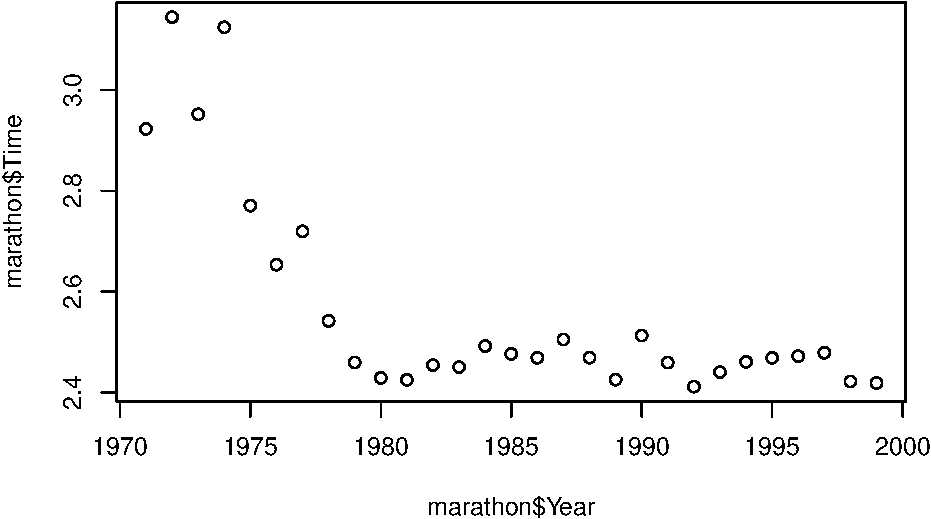
\includegraphics{RMarkdown-Example_files/figure-latex/unnamed-chunk-5-1.pdf}

or the time series plot:

\begin{Shaded}
\begin{Highlighting}[]
\KeywordTok{ts.plot}\NormalTok{(marathon}\OperatorTok{$}\NormalTok{Time)}
\end{Highlighting}
\end{Shaded}

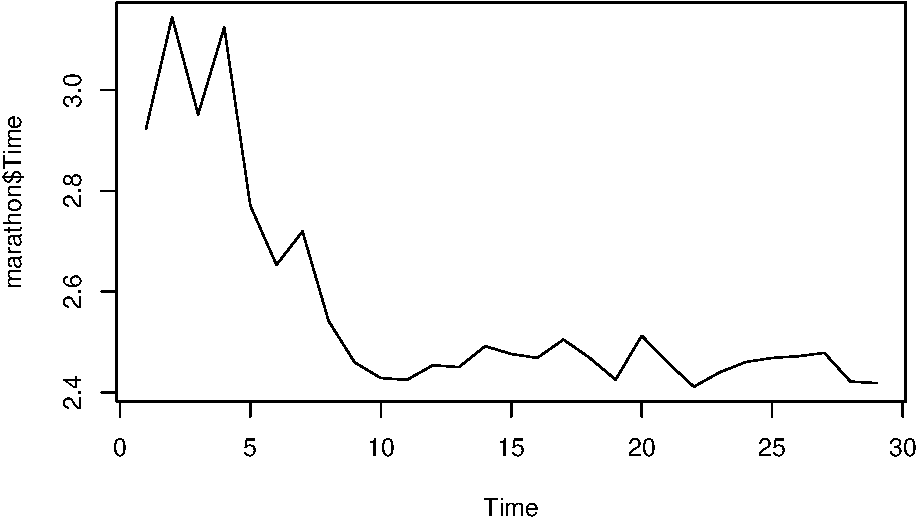
\includegraphics{RMarkdown-Example_files/figure-latex/unnamed-chunk-6-1.pdf}

\hypertarget{sleep-dataset}{%
\subsection{Sleep Dataset}\label{sleep-dataset}}

The Sleep dataset is a built-in dataset in R. Let us first gather some
information about this dataset.

\begin{Shaded}
\begin{Highlighting}[]
\KeywordTok{attributes}\NormalTok{(sleep)}
\end{Highlighting}
\end{Shaded}

\begin{verbatim}
## $names
## [1] "extra" "group" "ID"   
## 
## $class
## [1] "data.frame"
## 
## $row.names
##  [1]  1  2  3  4  5  6  7  8  9 10 11 12 13 14 15 16 17 18 19 20
\end{verbatim}

It has three columns, extra, group and ID.

Boxplot is a nice way to visualize the data, let us try for the extra
column: the increase in the number of hours of sleep resulting from
either drug.

\begin{Shaded}
\begin{Highlighting}[]
\KeywordTok{boxplot}\NormalTok{(sleep[}\StringTok{'extra'}\NormalTok{])}
\end{Highlighting}
\end{Shaded}

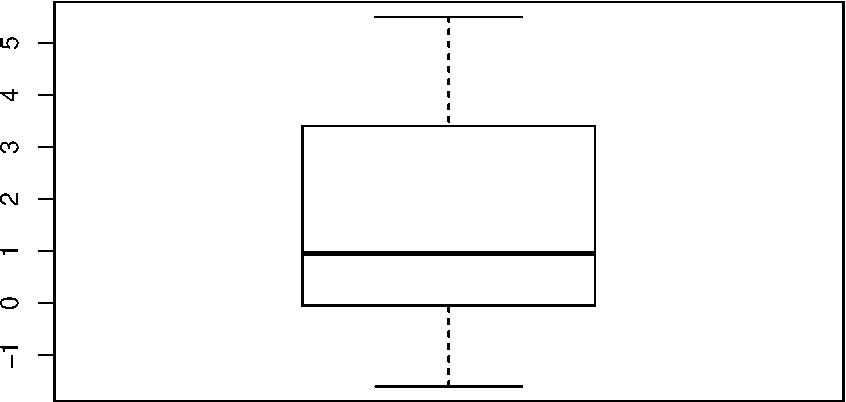
\includegraphics{RMarkdown-Example_files/figure-latex/unnamed-chunk-8-1.pdf}

In some data analysis, we need to focus on a subset of the data. For
instance, we want to separate group=1 and group=2. This can be achieved
using the following command:

\begin{Shaded}
\begin{Highlighting}[]
\NormalTok{group1 <-}\StringTok{ }\KeywordTok{subset}\NormalTok{(sleep,group}\OperatorTok{==}\DecValTok{1}\NormalTok{);}
\NormalTok{group2 <-}\StringTok{ }\KeywordTok{subset}\NormalTok{(sleep,group}\OperatorTok{==}\DecValTok{2}\NormalTok{)}
\end{Highlighting}
\end{Shaded}

We can check group1 and group 2:

\begin{Shaded}
\begin{Highlighting}[]
\NormalTok{group1}
\end{Highlighting}
\end{Shaded}

\begin{verbatim}
##    extra group ID
## 1    0.7     1  1
## 2   -1.6     1  2
## 3   -0.2     1  3
## 4   -1.2     1  4
## 5   -0.1     1  5
## 6    3.4     1  6
## 7    3.7     1  7
## 8    0.8     1  8
## 9    0.0     1  9
## 10   2.0     1 10
\end{verbatim}

\begin{Shaded}
\begin{Highlighting}[]
\NormalTok{group2}
\end{Highlighting}
\end{Shaded}

\begin{verbatim}
##    extra group ID
## 11   1.9     2  1
## 12   0.8     2  2
## 13   1.1     2  3
## 14   0.1     2  4
## 15  -0.1     2  5
## 16   4.4     2  6
## 17   5.5     2  7
## 18   1.6     2  8
## 19   4.6     2  9
## 20   3.4     2 10
\end{verbatim}

Now we can do a side by side comparison for the extra column between two
groups in order to understand the effects of these two types of drugs.

\begin{Shaded}
\begin{Highlighting}[]
\KeywordTok{boxplot}\NormalTok{(group1}\OperatorTok{$}\NormalTok{extra,group2}\OperatorTok{$}\NormalTok{extra)}
\end{Highlighting}
\end{Shaded}

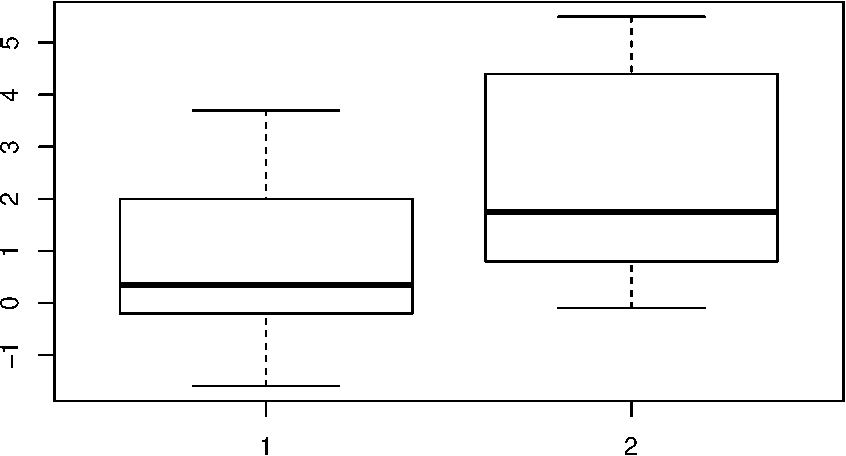
\includegraphics{RMarkdown-Example_files/figure-latex/unnamed-chunk-12-1.pdf}


\end{document}
